% ============================================================================
% A0 PORTRAIT POSTER (841mm x 1189mm) — pdfLaTeX / Overleaf-compatible
% "AI Agents for Data Visualization and Kaggle Competitions"
%
% Layout mirrors poster.html: navy top band, two columns of rounded cards
% with gold-underlined section titles.
%
% Compile with pdfLaTeX (Overleaf default). The only non-standard need is
% the CJK bsmi font (arphic) for the two Chinese names in the top band.
% ============================================================================
\documentclass{article}

% ---- Page geometry: exact A0 portrait, zero margins (we pad manually) ----
\usepackage[paperwidth=841mm,paperheight=1189mm,margin=0mm]{geometry}

\usepackage[T1]{fontenc}
\usepackage{helvet}                    % Helvetica clone, matches the HTML look
\renewcommand{\familydefault}{\sfdefault}
\usepackage{graphicx}
\usepackage{xcolor}
\usepackage{colortbl}                  % colored table rules
\usepackage{booktabs}                  % \specialrule in the results table
\usepackage{tikz}
\usepackage[skins]{tcolorbox}          % cards
\usepackage{enumitem}
\usepackage{textcomp}                  % \textperiodcentered
\usepackage{CJKutf8}                   % for the two Chinese names only

% ---- Palette (taken from poster.html) --------------------------------------
\definecolor{navy}{HTML}{0F2A4A}       % top band, headings
\definecolor{gold}{HTML}{E2B13C}       % accent rules / label accents
\definecolor{bandsub}{HTML}{BCD2EA}    % band subtitle
\definecolor{bandmeta}{HTML}{8FB0D4}   % band meta lines
\definecolor{cardborder}{HTML}{D5DBE3}
\definecolor{cardbg}{HTML}{FBFCFE}
\definecolor{bodyink}{HTML}{2A2E33}
\definecolor{boldblue}{HTML}{10365F}   % bold emphasis inside text
\definecolor{notegray}{HTML}{5A6472}   % captions / notes
\definecolor{barme}{HTML}{2B6CB0}      % highlighted bar (ours)
\definecolor{barother}{HTML}{A8BDD4}   % other bars
\definecolor{bartrack}{HTML}{EEF1F5}   % bar background track
\definecolor{tbdcol}{HTML}{8A6D1A}     % "TBD" highlight
\definecolor{footergray}{HTML}{7A8494}
\definecolor{ruleheavy}{HTML}{9FB0C4}  % table header rule
\definecolor{rulelight}{HTML}{DFE5EC}  % table row rule

% ---- Font sizes (pt), scaled from the HTML mm sizes ------------------------
\newcommand{\titlesize}{\fontsize{80}{90}\selectfont}
\newcommand{\subsize}{\fontsize{35}{45}\selectfont}
\newcommand{\metasize}{\fontsize{26}{36}\selectfont}
\newcommand{\cardtitlesize}{\fontsize{43}{50}\selectfont}
\newcommand{\subheadsize}{\fontsize{30.5}{37}\selectfont}
\newcommand{\bodysize}{\fontsize{26.5}{37.5}\selectfont}
\newcommand{\notesize}{\fontsize{22.5}{30}\selectfont}
\newcommand{\tablesize}{\fontsize{24}{33}\selectfont}
\newcommand{\footersize}{\fontsize{21}{28}\selectfont}

\renewcommand{\normalsize}{\bodysize}

% ---- Global layout params --------------------------------------------------
\setlength{\parindent}{0pt}
\setlength{\parskip}{0pt}
\setlength{\topskip}{0pt}
\setlength{\maxdepth}{\paperheight}    % the column row is one very deep line
\pagestyle{empty}

\newlength{\pagepad}\setlength{\pagepad}{21.25mm}   % outer horizontal padding
\newlength{\colgap}\setlength{\colgap}{9.55mm}      % gap between columns/cards

% ---- Helper macros ---------------------------------------------------------
% Bold emphasis in body text (HTML <b> is dark blue)
\newcommand{\kb}[1]{\textbf{\textcolor{boldblue}{#1}}}
% Separator dot for meta/footer lines
\newcommand{\sep}{\ \textperiodcentered\ }

% Card container
\newtcolorbox{card}{%
  enhanced, sharp corners=all, arc=4.26mm, rounded corners=all,
  colback=cardbg, colframe=cardborder, boxrule=0.85mm,
  left=11.5mm, right=11.5mm, top=11mm, bottom=12mm, boxsep=0pt,
  before skip=0pt, after skip=\colgap}

% Card section title: navy, gold underline
\newcommand{\cardtitle}[1]{%
  {\cardtitlesize\bfseries\color{navy}#1\par}%
  \vspace{3.2mm}{\color{gold}\rule{\linewidth}{1.27mm}}\par\vspace{5.5mm}}

% Card sub-heading (h3)
\newcommand{\cardsub}[1]{%
  \vspace{4.5mm}{\subheadsize\bfseries\color{navy}#1\par}\vspace{2.8mm}}

% Figure caption
\newcommand{\figcap}[1]{\vspace{2mm}{\notesize\color{notegray}#1\par}}
% Note paragraph
\newcommand{\notepar}[1]{{\notesize\color{notegray}#1\par}}

% Bullet list defaults
\setlist[itemize]{leftmargin=11mm, itemsep=4.2mm, parsep=0pt, topsep=1.5mm,
                  label=\textbullet}

% ---- Horizontal bar row for the SMAPE ablation chart -----------------------
% Bars are proportional to the margin over 52 (lower SMAPE is better),
% i.e. bar length = (52 - value)/5 of the full track (matches the HTML).
% #1 = label, #2 = bar color, #3 = fraction of track (0..1), #4 = value text
\newlength{\bartracklen}\setlength{\bartracklen}{235mm}
\newcommand{\smapebar}[4]{%
  \makebox[64mm][l]{\bodysize #1}%
  \begin{tikzpicture}[baseline={(0,4.2mm)}]
    \fill[bartrack, rounded corners=2.12mm] (0,0) rectangle (\bartracklen,13.3mm);
    \fill[#2, rounded corners=2.12mm] (0,0) rectangle (#3\bartracklen,13.3mm);
  \end{tikzpicture}%
  \hspace{3mm}{\tablesize\color{bodyink}#4}\par\vspace{3.6mm}}

% ============================================================================
\begin{document}%
\bodysize\color{bodyink}%

% ---------------------------------------------------------------- TOP BAND --
\begin{tcolorbox}[enhanced, width=\paperwidth, sharp corners,
    colback=navy, boxrule=0pt, frame hidden,
    left=\pagepad, right=\pagepad, top=17mm, bottom=15mm, boxsep=0pt,
    before skip=0pt, after skip=0pt]
  {\titlesize\bfseries\color{white}%
    AI Agents for Data Visualization and Kaggle Competitions\par}
  \vspace{5.3mm}
  {\subsize\color{bandsub}%
    An end-to-end LLM agent (my-agent) benchmarked against two frozen
    yardsticks on 20 Kaggle competitions --- with the apparatus needed to
    make the comparison honest\par}
  \vspace{4.3mm}
  {\metasize\color{bandmeta}%
    {\bfseries\color{gold}Author:} Wei-Hao Huang
    (\begin{CJK}{UTF8}{bsmi}黃威昊\end{CJK})\sep
    {\bfseries\color{gold}School:} National Chengchi University,
    Department of Economics\par}
  \vspace{2.5mm}
  {\metasize\color{bandmeta}%
    {\bfseries\color{gold}Advisor:} Dr.\ Tso-Jung Yen
    (\begin{CJK}{UTF8}{bsmi}顏佐榕\end{CJK}),
    Institute of Statistical Science, Academia Sinica\sep
    Summer Internship 2026\par}
\end{tcolorbox}

\vspace{11.7mm}

% ------------------------------------------------------------- BODY COLUMNS --
\noindent\hspace*{\pagepad}%
%
% ============================== LEFT COLUMN (379.3mm) ======================
\begin{minipage}[t]{379.3mm}
\vspace{0pt}% anchor the column reference point at its top

% ---- 1 · Motivation --------------------------------------------------------
\begin{card}
\cardtitle{1\sep Motivation}
\cardsub{Why these tasks are hard}
\begin{itemize}
  \item \kb{Kaggle competitions} demand the full expert loop --- validation
    design, feature engineering, model selection, ensembling --- where the
    difference between top entries sits at the \kb{4th--5th decimal} of the
    metric.
  \item With gaps that small, \kb{local cross-validation is an unreliable
    compass}: a pipeline's own validation score routinely disagrees with the
    real leaderboard, so no local number can be trusted to pick a winner.
  \item \kb{Data visualization} (EDA, diagnostics, reporting) is essential
    but repetitive: every dataset needs distribution, drift, and correlation
    views before modeling can be trusted.
\end{itemize}
\cardsub{Why an AI agent}
\begin{itemize}
  \item Tireless, systematic search: 22--80 candidate configurations per
    competition, every experiment logged and reproducible.
  \item Runs the same disciplined protocol on 20 competitions serially ---
    a human cannot hold this consistency.
  \item Generates per-dataset EDA figures and per-competition reports
    automatically, so every claim is grounded in an artifact.
\end{itemize}
\end{card}

% ---- 2 · Workflow ----------------------------------------------------------
\begin{card}
\cardtitle{2\sep Workflow}
An LLM reasons at every stage; Auto-ML libraries are invoked through the
shell; a cross-competition \kb{experience library} supplies evidence-backed
priors; a \kb{tree search} over candidate configurations is the optimisation
loop.\par
\vspace{4mm}

\includegraphics[width=\linewidth]{fig1_arch.pdf}
\figcap{Six-stage pipeline: problem dossier $\to$ EDA $\to$ features $\to$
  modeling $\to$ evaluation $\to$ submission. The v5 dossier layer classifies
  the task and injects external data \emph{upstream}, before any modeling.}
\vspace{4mm}
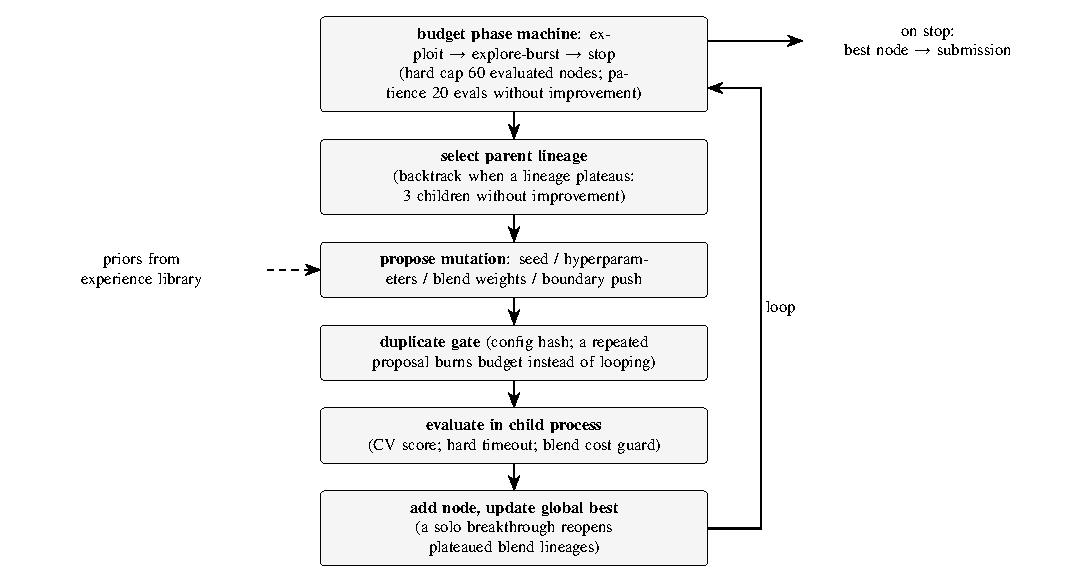
\includegraphics[width=\linewidth]{fig2_tree.pdf}
\figcap{Tree-search loop: ensembles are first-class nodes with OOF caching
  and weight search; exploit until plateau, then one forced exploration
  burst.}
\end{card}

\end{minipage}%
\hspace{\colgap}%
%
% ============================== RIGHT COLUMN (409.65mm) ====================
\begin{minipage}[t]{409.65mm}
\vspace{0pt}% anchor the column reference point at its top

% ---- 3 · Results — Kaggle benchmark ---------------------------------------
\begin{card}
\cardtitle{3\sep Results --- Kaggle benchmark}
\notepar{All submissions scored on the real leaderboard (late submission);
  verdicts adjudicated by a paired test built from Kaggle's own
  public/private split.}
\cardsub{Benchmark standing (scored 2026-08-18, 16 of 20 lanes)}
All 20 competitions run under the frozen Stage-0.5 architecture in
credential-free sandboxes with a per-lane transcript audit. The 16 completed
lanes are scored on the real leaderboard, each duel adjudicated by a paired
test built from Kaggle's own public/private split: \kb{my-agent leads the
standing --- 15 wins / 5 losses (75\% excl.\ ties)} vs.\ AIDE 42\% and NVIDIA
38\% --- and takes the \kb{best private score on 10 of 16}. One lane running
(s6e2), three queued ({\bfseries\color{tbdcol}TBD}).\par
\cardsub{Injection-layer ablation (s3e19, private SMAPE $\downarrow$)}
% Bar lengths proportional to margin over 52: (52 - SMAPE)/5 of the track.
\smapebar{\kb{with layer}}{barme}{0.7514}{48.243}
\smapebar{NVIDIA}{barother}{0.7469}{48.26558}
\smapebar{AIDE}{barother}{0.7317}{48.34131}
\smapebar{no layer}{barother}{0.3090}{50.455}
\notepar{The dossier layer's external-data injection turns the
  architecture's canonical failure into a numerical first among the three
  agents --- and all \kb{6 of 6} controlled external-data arms beat their
  matched baselines. Bar length $\propto$ margin over 52 (lower SMAPE is
  better).}
\cardsub{Mid-complexity three-way (offline-graded, private split)}
{\tablesize
\renewcommand{\arraystretch}{1.55}%
\setlength{\tabcolsep}{2.6mm}%
\begin{tabular}{@{}l l r r r@{}}
  \arrayrulecolor{ruleheavy}%
  {\color{notegray}Competition} & {\color{notegray}Metric} &
    {\color{notegray}my-agent} & {\color{notegray}NVIDIA} &
    {\color{notegray}AIDE}\\
  \specialrule{0.74mm}{1mm}{1mm}%
  \arrayrulecolor{rulelight}%
  us-patent (NLP) & Pearson $r$ $\uparrow$ &
    \kb{0.86658} & 0.86160 & 0.65821\\ \specialrule{0.37mm}{0.8mm}{0.8mm}
  ventilator (time series) & MAE $\downarrow$ &
    \kb{0.16525} & 0.40093 & 0.34591\\ \specialrule{0.37mm}{0.8mm}{0.8mm}
  SIIM-ISIC (imaging) & AUC $\uparrow$ &
    \kb{0.93529} & 0.89822 & 0.88579\\ \specialrule{0.37mm}{0.8mm}{0.8mm}
\end{tabular}\par}
\end{card}

% ---- 4 · Advantages & Difficulties ----------------------------------------
\begin{card}
\cardtitle{4\sep Advantages \& Difficulties}
\cardsub{Expected $\to$ experienced}
\begin{itemize}
  \item \kb{Expected:} the agent would quickly beat most humans.
    \kb{Experienced:} development runs landed above average, with wins
    concentrated where no mature public solutions exist; the
    frozen-architecture re-run now leads the paired standing on the 16
    scored lanes.
  \item \kb{Expected:} one run and one score decide a winner.
    \kb{Experienced:} score noise and run-to-run variance leave many duels
    undecidable; a paired error model became mandatory.
  \item \kb{Expected:} the agent follows the rules by default.
    \kb{Experienced:} a transcript audit caught one lane reading its own
    competition's recorded findings --- and the clean re-run scored
    \emph{worse}, proving the contamination advantage was real.
  \item Fairness is expensive: isolated data roots, credential-free
    sandboxes, and per-lane transcript audits cost real engineering time ---
    but without them the numbers are not comparable.
\end{itemize}
\end{card}

% ---- 5 · Discussion — advice ----------------------------------------------
\begin{card}
\cardtitle{5\sep Discussion --- advice}
\begin{itemize}
  \item \kb{State the error model with every claim.} A ranking without an
    error scale is noise: many of our duels are undecidable, and the winner
    flips when the evaluation set changes.
  \item \kb{Never trust local CV for between-agent claims.} Score on the
    real leaderboard; CV describes a pipeline's internal view only.
  \item \kb{Freeze your yardsticks.} Improving a baseline mid-study silently
    turns the benchmark into an optimisation of the baseline.
  \item \kb{Isolate mechanically, then audit the transcript.} Sandboxes stop
    leaks you anticipated; reading what the agent actually did catches the
    ones you didn't --- in both directions (we hit one real contamination
    and one auditor false positive).
  \item \kb{Put knowledge injection upstream.} Injected at the blend stage
    it was worth ${\sim}10^{-5}$; moved into problem identification it
    lifted the canonical failure case from last to first.
\end{itemize}
\cardsub{Where knowledge enters}
\begin{itemize}
  \item Downstream (blend stage): measured gain ${\sim}10^{-5}$ ---
    abandoned.
  \item Upstream (problem dossier): fires on exactly the \kb{2/18}
    competitions that need external data; all \kb{6 of 6} controlled
    external-data arms beat their matched baselines.
  \item But no local signal can select the \emph{form} of injection --- the
    one surviving selector died on its first pre-registered prediction.
\end{itemize}
\vspace{3mm}
\notepar{Companion documents: Report v6 (Overleaf, main document)\sep
  Engineering Log\sep Case Studies\sep 22 per-competition ML-spec reports.}
\end{card}

\end{minipage}

% ------------------------------------------------------------------ FOOTER --
\vfill
\noindent\hspace*{\pagepad}%
\begin{minipage}{798.5mm}
  {\footersize\color{footergray}%
    All numbers are real measurements as of 2026-08-18 (16 of 20 re-run
    lanes scored on the real leaderboard; four lanes still to finish)\sep
    AIDE = LLM tree search; NVIDIA = highest-voted-kernel reproduction,
    both frozen.\par}
\end{minipage}
\vspace{9.5mm}

\end{document}
